\documentclass[10pt,aspectratio=169,professionalfonts]{beamer}
\usetheme[progressbar=frametitle,block=fill,numbering=fraction]{metropolis}

\usepackage{appendixnumberbeamer}
\usepackage{booktabs}
\usepackage{amsmath,amssymb,mathtools}
\usepackage{siunitx}
\usepackage{tikz}
\usetikzlibrary{calc,arrows.meta,shapes,positioning,decorations.pathmorphing,patterns}
\usepackage{pgfplots}
\pgfplotsset{compat=1.17}
\usepackage{xcolor}
\usepackage{graphicx}
\usepackage{array,multirow}

%% ─── colours ────────────────────────────────────────────────────────────────
\definecolor{mblue}{HTML}{2c7bb6}
\definecolor{mred}{HTML}{d73027}
\definecolor{mgreen}{HTML}{1a9850}
\definecolor{morange}{HTML}{f46d43}
\definecolor{mgray}{HTML}{aaaaaa}
\definecolor{mdblue}{HTML}{08519c}
\definecolor{mlblue}{HTML}{9ecae1}

\setbeamercolor{palette primary}{bg=mblue,fg=white}
\setbeamercolor{progress bar}{fg=mblue,bg=mlblue}
\setbeamercolor{alerted text}{fg=mred}
\setbeamercolor{block title alerted}{fg=white,bg=mred}

%% ─── math shorthands ────────────────────────────────────────────────────────
\newcommand{\Esta}{E^*}
\newcommand{\pbar}{\bar{p}}
\newcommand{\diag}{\mathrm{diam}}
\newcommand{\dist}{\mathrm{dist}}
\newcommand{\calL}{\mathcal{L}}
\newcommand{\T}{\mathsf{T}}

%% ─── tikz styles ────────────────────────────────────────────────────────────
\tikzset{
  leaf/.style={fill=mlblue!40,draw=mblue,rounded corners=1pt},
  block lr/.style={fill=mlblue,opacity=0.6},
  block d/.style={fill=mgray!50},
  arr/.style={->,>=Stealth,thick,mblue},
}

%% ─── title info ─────────────────────────────────────────────────────────────
\title{H-Matrix BEM for Rough-Surface\\Normal Contact}
\subtitle{Non-periodic solver · Love element integration · Polonsky--Keer PCG}
\author{V.~Yastrebov}
\institute{MINES Paris -- PSL, Centre des Mat\'eriaux}
\date{2026}

\begin{document}

\maketitle

%% ── Section §1: H-matrix solver ─────────────────────────────────────────────
%% §1 — H-Matrix BEM Solver  (5 slides)
\section{H-Matrix BEM Solver}

%% ── Slide 1: The N² wall ────────────────────────────────────────────────────
\begin{frame}{The $N^2$ Wall}
\begin{columns}[T]
\begin{column}{0.48\textwidth}
  Surface contact requires \textbf{dense matrix–vector products}
  \[
    u_i = \sum_{j=1}^{N} S_{ij}\,p_j,
    \qquad S_{ij} = \frac{1}{\pi\Esta}
      \calL\!\left(\mathbf{x}_i{-}\mathbf{x}_j,\tfrac{h}{2}\right)
  \]
  \begin{block}{Cost of dense BEM ($N = N_s^2$)}
    \begin{tabular}{lcc}
      \toprule
      Operation & Time & Memory \\
      \midrule
      Assembly  & $O(N^2)$ & $8N^2$ bytes \\
      Matvec    & $O(N^2)$ & \\
      \bottomrule
    \end{tabular}
  \end{block}
  \vspace{0.4em}
  \textbf{Concrete}: $N_s=256$ ($N=65\,536$)
  $\;\Rightarrow\;$ \alert{34\,GB} just to store $S$
\end{column}
\begin{column}{0.48\textwidth}
  \begin{block}{H-matrix target}
    \begin{tabular}{lc}
      \toprule
      Operation & Cost \\
      \midrule
      Assembly  & $O(N\log^2 N)$ \\
      Matvec    & $O(N\log N)$ \\
      Memory    & $\ll N^2$ \\
      \bottomrule
    \end{tabular}
  \end{block}
  \vspace{0.4em}
  Key idea: \textbf{far-field interactions are low-rank}
  \[
    S[I,J] \approx UV^\T, \quad k \ll |I|,|J|
  \]
\end{column}
\end{columns}
\end{frame}

%% ── Slide 2: Quad-tree cluster tree ─────────────────────────────────────────
\begin{frame}{Cluster Tree: Quad-Tree on the 2D Grid}
\begin{columns}[T]
\begin{column}{0.45\textwidth}
  \begin{itemize}
    \item Recursively split $N_s\!\times\!N_s$ grid at midpoints
    \item Each node owns a contiguous \textbf{permuted} index range
    \item Leaves hold $\le$ \texttt{leaf\_size} elements
    \item Depth $\le \log_4 N$
  \end{itemize}
  \vspace{0.8em}
  \textbf{Geometry} (Chebyshev distance):
  \[
    \diag(t)   = \max(\Delta i_x, \Delta i_y)
  \]
  \[
    \dist(t,s) = \max(d_x^+, d_y^+)\;\ge 0
  \]
\end{column}
\begin{column}{0.50\textwidth}
  \centering
  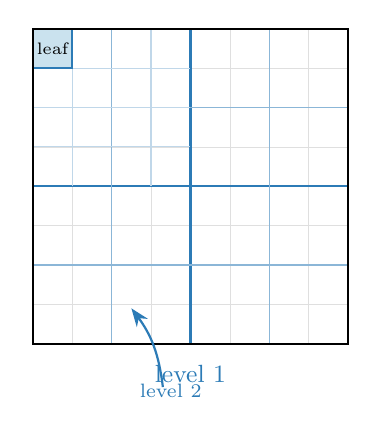
\begin{tikzpicture}[scale=0.50]
    % background grid
    \foreach \x in {0,...,8}
      \draw[gray!25,very thin] (\x,0)--(\x,8);
    \foreach \y in {0,...,8}
      \draw[gray!25,very thin] (0,\y)--(8,\y);
    % Level 1 splits
    \draw[mblue,thick] (4,0)--(4,8) (0,4)--(8,4);
    % Level 2 splits
    \foreach \x/\ya/\yb in {2/0/4, 6/0/4, 2/4/8, 6/4/8}
      \draw[mblue!55] (\x,\ya)--(\x,\yb);
    \foreach \y/\xa/\xb in {2/0/4, 6/0/4, 2/4/8, 6/4/8}
      \draw[mblue!55] (\xa,\y)--(\xb,\y);
    % Level 3 (top-left quadrant only)
    \draw[mblue!30] (1,4)--(1,8) (3,4)--(3,8)
                    (0,5)--(4,5) (0,7)--(4,7)
                    (1,6)--(1,8) (3,6)--(3,8)
                    (0,6)--(2,6) (2,6)--(4,6);
    % Highlighted leaf
    \fill[mlblue!55,draw=mblue,line width=0.6pt] (0,7) rectangle (1,8);
    \node[font=\fontsize{6}{7}\selectfont] at (0.5,7.5) {leaf};
    % border
    \draw[black,thick] (0,0) rectangle (8,8);
    % labels
    \node[below,font=\small,mblue] at (4,-0.3) {level 1};
    \draw[arr] (3.3,-1.1) to[bend right=15] (2.5,0.9);
    \node[font=\fontsize{7}{8}\selectfont,mblue] at (3.5,-1.2) {level 2};
  \end{tikzpicture}
\end{column}
\end{columns}
\end{frame}

%% ── Slide 3: Admissibility and block partition ──────────────────────────────
\begin{frame}{Admissibility Condition \& Block Partition}
\begin{columns}[T]
\begin{column}{0.44\textwidth}
  Block $(t,s)$ is \textbf{admissible} (low-rank) when:
  \[
    \min\!\bigl(\diag(t),\diag(s)\bigr)
    \;\le\; \eta\,\dist(t,s),
    \quad \eta=2
  \]
  Otherwise (near-diagonal): \textbf{dense} block.

  \vspace{0.6em}
  \textbf{ACA fill} (admissible blocks):
  \[
    S[I,J] \approx UV^\T
  \]
  Stop when $\|u_k\|\|v_k\| \le \varepsilon_{\rm aca}\,\|A_k\|_F$

  \vspace{0.4em}
  Typical rank $k\approx 11$ at $N_s=64$
\end{column}
\begin{column}{0.52\textwidth}
  \centering
  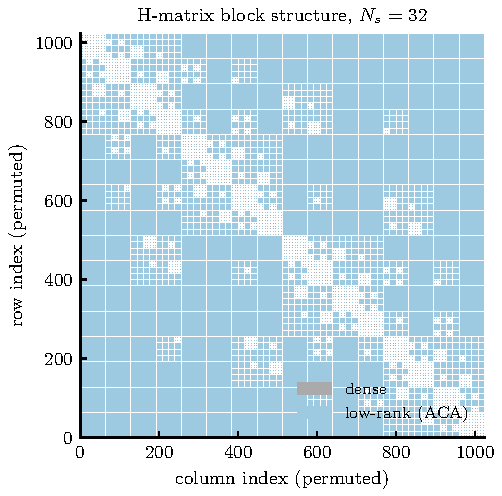
\includegraphics[width=0.94\linewidth]{figures/fig_hmatrix_blocks.pdf}
\end{column}
\end{columns}
\end{frame}

%% ── Slide 4: H-matrix matvec ────────────────────────────────────────────────
\begin{frame}{H-Matrix Matrix–Vector Product}
\begin{columns}[T]
\begin{column}{0.50\textwidth}
  \textbf{Block loop} (OpenMP parallel):
  \vspace{0.3em}

  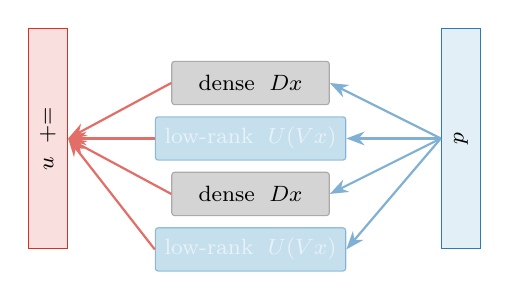
\begin{tikzpicture}[node distance=4pt]
    % blocks
    \node[block d, minimum width=2.0cm, minimum height=0.55cm,
          draw=mgray, rounded corners=1pt] (d1) {\footnotesize dense $\;D x$};
    \node[block lr, minimum width=2.0cm, minimum height=0.55cm,
          below=of d1, draw=mblue!80, rounded corners=1pt]
         (lr1) {\footnotesize\color{white}low-rank $\;U(Vx)$};
    \node[block d, minimum width=2.0cm, minimum height=0.55cm,
          below=of lr1, draw=mgray, rounded corners=1pt]
         (d2) {\footnotesize dense $\;D x$};
    \node[block lr, minimum width=2.0cm, minimum height=0.55cm,
          below=of d2, draw=mblue!80, rounded corners=1pt]
         (lr2) {\footnotesize\color{white}low-rank $\;U(Vx)$};
    % p vector
    \node[draw=mblue, minimum width=0.5cm, minimum height=2.8cm,
          right=1.2cm of lr1, fill=mlblue!30] (pv)
         {\rotatebox{90}{\footnotesize $p$}};
    % u vector
    \node[draw=mred, minimum width=0.5cm, minimum height=2.8cm,
          left=1.1cm of lr1, fill=mred!15] (uv)
         {\rotatebox{90}{\footnotesize $u\;\mathrel{+}=$}};
    % arrows
    \foreach \blk in {d1,lr1,d2,lr2}{
      \draw[arr,mblue!60] (pv.west) -- (\blk.east);
      \draw[arr,mred!70]  (\blk.west) -- (uv.east);
    }
  \end{tikzpicture}
\end{column}
\begin{column}{0.46\textwidth}
  \[
    u(I) \mathrel{+}= D\,p(J) \quad\text{(dense)}
  \]
  \[
    u(I) \mathrel{+}= U\bigl(V\,p(J)\bigr) \quad\text{(low-rank)}
  \]
  \vspace{0.5em}
  \begin{itemize}
    \item Permute $p$ once before the loop
    \item Each block is \textbf{independent} $\to$ OpenMP
    \item Complexity: $O(N\log^2 N)$
  \end{itemize}
  \vspace{0.4em}
  \textbf{Measured}: $N\!=\!4096$ ($N_s\!=\!64$)\\
  \hspace{1em} assembly: 7\,ms \;|\; matvec: 0.6\,ms
\end{column}
\end{columns}
\end{frame}

%% ── Slide 5: Boussinesq kernel (Love formula) ────────────────────────────────
\begin{frame}{Boussinesq Green's Function: Love Element Formula}
\begin{columns}[T]
\begin{column}{0.54\textwidth}
  Green's function for elastic half-space ($\Esta = E/(1-\nu^2)$):
  \[
    G(\mathbf{r}) = \frac{1}{\pi\Esta |\mathbf{r}|}
  \]
  Discretise on $N_s\!\times\!N_s$ grid of elements of side $h$:
  \[
    S_{ij} = \frac{1}{\pi\Esta}\,\calL\!\left(\Delta x,\Delta y,\tfrac{h}{2}\right)
  \]
  \textbf{Love (1929)} exact integral over a square element:
  {\small
  \begin{align*}
    \calL(x,y,a) &= (x{+}a)\ln\frac{(y{+}a)+R_{++}}{(y{-}a)+R_{+-}}
                 +(y{+}a)\ln\frac{(x{+}a)+R_{++}}{(x{-}a)+R_{-+}} \\
                 &\quad+(x{-}a)\ln\frac{(y{-}a)+R_{--}}{(y{+}a)+R_{-+}}
                 +(y{-}a)\ln\frac{(x{-}a)+R_{--}}{(x{+}a)+R_{+-}}
  \end{align*}
  }
  \alert{Self-term}: $S_{ii} = \dfrac{4h\ln(1{+}\sqrt{2})}{\pi\Esta}$
\end{column}
\begin{column}{0.42\textwidth}
  \centering
  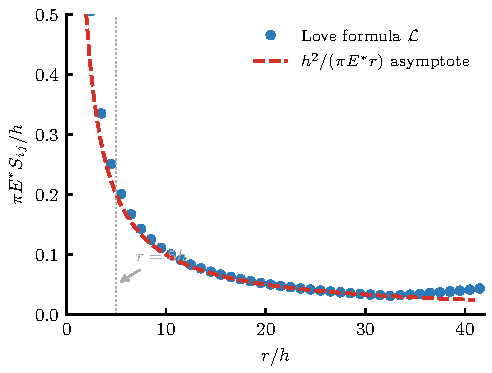
\includegraphics[width=\linewidth]{figures/fig_kernel_decay.pdf}
  \vspace{0.3em}
  {\small 3.7\,\% deviation at $r=h$; below 0.2\,\% at $r\ge5h$}
\end{column}
\end{columns}
\end{frame}


%% ── Section §2: Hertz problem ───────────────────────────────────────────────
%% §2 — The Hertz Problem  (4 slides)
\section{The Hertz Problem}

%% ── Slide 6: Geometry ───────────────────────────────────────────────────────
\begin{frame}{Hertz Contact: Problem Setup}
\begin{columns}[T]
\begin{column}{0.44\textwidth}
  \centering
  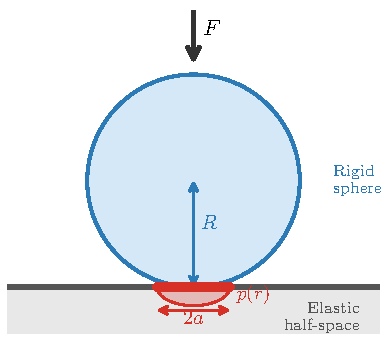
\includegraphics[width=0.88\linewidth]{figures/fig_hertz_geometry.pdf}
\end{column}
\begin{column}{0.52\textwidth}
  \textbf{Rigid sphere} (radius $R$) pressed onto an
  \textbf{elastic half-space} ($\Esta$) with total load $F$.
  \vspace{0.6em}

  Parabolic \textbf{initial gap}:
  \[
    g_0(r) = \frac{r^2}{2R}, \qquad r = \sqrt{x^2+y^2}
  \]
  \textbf{Unknowns}: contact pressure $p(\mathbf{x})$,
  contact radius $a$, approach $\delta$.

  \vspace{0.5em}
  \begin{block}{Boundary conditions in contact ($r<a$)}
    $p \ge 0,\quad u_z = \delta - g_0 \ge 0$
  \end{block}
  \begin{block}{Outside contact ($r\ge a$)}
    $p = 0,\quad u_z < \delta - g_0$
  \end{block}
\end{column}
\end{columns}
\end{frame}

%% ── Slide 7: Analytical solution ────────────────────────────────────────────
\begin{frame}{Hertz Analytical Solution}
\begin{columns}[T]
\begin{column}{0.48\textwidth}
  \textbf{Contact radius}:
  \[
    a = \left(\frac{3FR}{4\Esta}\right)^{1/3}
  \]
  \textbf{Hertzian pressure distribution}:
  \[
    p(r) = p_0\sqrt{1 - \left(\frac{r}{a}\right)^2},
    \quad r \le a
  \]
  \textbf{Peak pressure}:
  \[
    p_0 = \frac{3F}{2\pi a^2}
  \]
  \textbf{Indentation}:
  \[
    \delta = \frac{a^2}{R}
  \]
\end{column}
\begin{column}{0.48\textwidth}
  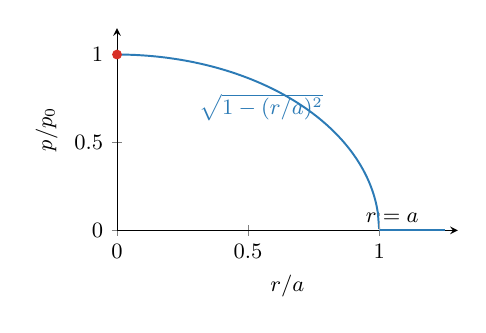
\begin{tikzpicture}[scale=0.88]
    % Hertz pressure half-arch sketch
    \begin{axis}[
      width=6.5cm, height=4.5cm,
      axis lines=left,
      xlabel={$r/a$}, ylabel={$p/p_0$},
      xmin=0, xmax=1.3, ymin=0, ymax=1.15,
      xtick={0,0.5,1.0},
      ytick={0,0.5,1.0},
      tick label style={font=\small},
      label style={font=\small},
      clip=false,
    ]
    \addplot[domain=0:1, samples=200, thick, mblue]
      {sqrt(max(0,1-x*x))};
    \addplot[domain=1:1.25, samples=5, thick, mblue]
      {0};
    \addplot[only marks, mark=*, mark size=1.8pt, mred]
      coordinates {(0,1)};
    \draw[dashed,mgray] (axis cs:1,0) -- (axis cs:1,0.1);
    \node[font=\small] at (axis cs:1.05,0.07) {$r=a$};
    \node[font=\small,mblue] at (axis cs:0.55,0.7)
      {$\sqrt{1-(r/a)^2}$};
    \end{axis}
  \end{tikzpicture}
\end{column}
\end{columns}
\end{frame}

%% ── Slide 8: BEM discretisation + Polonsky–Keer ─────────────────────────────
\begin{frame}{BEM Discretisation \& Polonsky--Keer Algorithm}
\begin{columns}[T]
\begin{column}{0.50\textwidth}
  Grid $N_s\!\times\!N_s$, element size $h=L/N_s$, flat index $k=i_y N_s+i_x$:
  \[
    S_{ij} = \frac{\calL(\mathbf{x}_i - \mathbf{x}_j,\;h/2)}{\pi\Esta}
  \]
  \vspace{-0.3em}
  \textbf{Contact QP}:
  \[
    \min_{p}\;\tfrac{1}{2}p^\T Sp + p^\T g_0
    \;\text{s.t.}\;p_i\ge0,\;\bar p = p_{\rm nom}
  \]
\end{column}
\begin{column}{0.46\textwidth}
  \begin{block}{Polonsky--Keer (1999) PCG}
    \small
    \begin{enumerate}
      \item Init $p = \pbar\mathbf{1}$; $u = Sp$; $r = u+g_0$
      \item Shift: $\bar r = r - \langle r\rangle_{\rm contact}$
      \item Zero $r_i$ if $p_i=0$ and $\bar r_i \ge 0$
      \item $\delta = \|r\|^2$; \textbf{converge} if $\delta<\varepsilon^2\delta_0$
      \item $t = r + (\delta/\delta_{\rm old})\,t$; mask $t$
      \item $v=St$;\; $\tau = \langle r,t\rangle/\langle v,t\rangle_{\rm c}$
      \item $p \mathrel{-}= \tau t$;\; $p \leftarrow \max(p,0)$
      \item Overlap correction;\; normalise $p$
      \item $u = Sp$;\; $r = u+g_0$
    \end{enumerate}
  \end{block}
\end{column}
\end{columns}
\end{frame}

%% ── Slide 9: Hertz validation ───────────────────────────────────────────────
\begin{frame}{Hertz Validation ($N_s=64$, $\Esta=1$, $R=0.5$)}
  \centering
  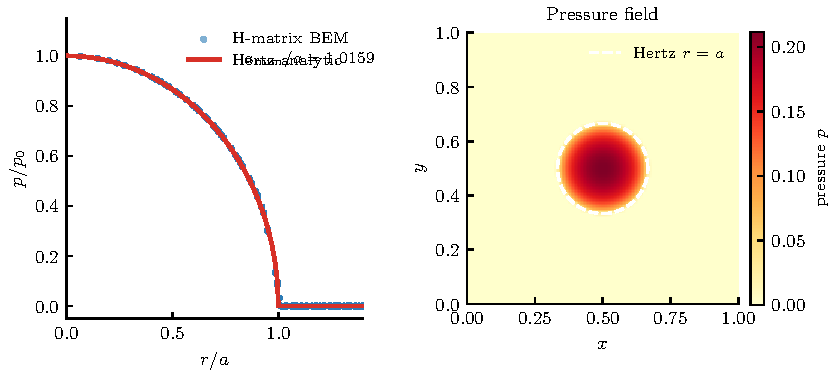
\includegraphics[width=0.92\linewidth]{figures/fig_hertz_validation.pdf}
  \vspace{0.3em}

  \begin{columns}
  \begin{column}{0.48\textwidth}
    \centering
    {\small
    $a_{\rm num}/a_{\rm Hertz} = 1.016$ \quad
    $p_{\rm max}/p_0 = 0.998$
    }
  \end{column}
  \begin{column}{0.48\textwidth}
    \centering
    {\small
    Mean pressure error $< 10^{-10}$\quad
    Converged in 29 iterations
    }
  \end{column}
  \end{columns}
\end{frame}


%% ── Section §3: Rough surface contact ──────────────────────────────────────
%% §3 — Rough Surface Contact  (4 slides)
\section{Rough Surface Contact}

%% ── Slide 10: Real surfaces are rough ───────────────────────────────────────
\begin{frame}{Real Surfaces are Multi-Scale Rough}
\begin{columns}[T]
\begin{column}{0.50\textwidth}
  \textbf{Self-affine surfaces}: statistically scale-invariant
  \[
    C(q) \sim q^{-2(1+H)},\quad H\in(0,1)
  \]
  ($H$ = Hurst exponent, $q$ = spatial frequency)

  \vspace{0.5em}
  Profile sketch (three-scale superposition):
  \vspace{0.2em}

  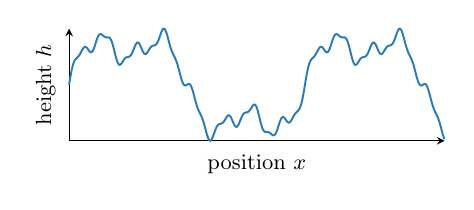
\begin{tikzpicture}[scale=0.88]
    \begin{axis}[
      width=7cm, height=3.2cm,
      axis lines=left,
      xlabel={position $x$}, ylabel={height $h$},
      xtick=\empty, ytick=\empty,
      label style={font=\small},
      clip=false,
    ]
    \addplot[domain=0:10,samples=400,thick,mblue]
      {0.55*sin(deg(x)) + 0.22*sin(3*deg(x)) + 0.10*sin(8*deg(x))
       + 0.04*sin(18*deg(x))};
    \end{axis}
  \end{tikzpicture}
\end{column}
\begin{column}{0.46\textwidth}
  \centering
  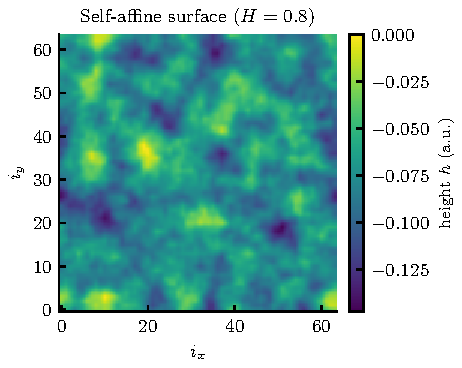
\includegraphics[width=0.94\linewidth]{figures/fig_surface.pdf}

  \vspace{0.3em}
  {\small $N_s=64$, $H=0.8$, seed 12345\\
  normalised: RMS slope $= 1$}
\end{column}
\end{columns}
\end{frame}

%% ── Slide 11: Contact problem as QP ────────────────────────────────────────
\begin{frame}{Normal Contact as a Quadratic Programme}
\begin{columns}[T]
\begin{column}{0.50\textwidth}
  \textbf{Influence matrix}: $u = Sp$, symmetric PSD ($N\!\times\!N$)

  \textbf{Complementarity energy}:
  \[
    W(p) = \frac{1}{2}p^\T S p + p^\T g_0
  \]

  \textbf{Minimise} subject to:
  \[
    p_i \ge 0 \quad\forall i, \qquad
    \frac{1}{N}\sum_i p_i = \pbar
  \]

  \vspace{0.3em}
  \textbf{KKT conditions} (complementarity):
  \[
    (Sp+g_0)_i \ge 0,\quad p_i \ge 0
  \]
  \[
    p_i\,(Sp+g_0)_i = 0
  \]
\end{column}
\begin{column}{0.46\textwidth}
  \begin{block}{Physical meaning}
    \begin{itemize}
      \item $p_i > 0$: element \emph{in contact}
        $\Rightarrow$ gap $= 0$
      \item $p_i = 0$: element \emph{not in contact}
        $\Rightarrow$ gap $\ge 0$
    \end{itemize}
  \end{block}
  \vspace{0.4em}
  \begin{alertblock}{No-penetration + non-adhesion}
    $g_i = u_i + g_{0,i} - \delta \ge 0$ everywhere,\\
    with $\delta$ the rigid-body approach.
  \end{alertblock}
\end{column}
\end{columns}
\end{frame}

%% ── Slide 12: Full Polonsky–Keer algorithm ──────────────────────────────────
\begin{frame}{Polonsky--Keer Projected CG (full)}
\begin{columns}[T]
\begin{column}{0.50\textwidth}
  \begin{block}{Initialisation}
    $p \leftarrow \pbar\mathbf{1}$;\quad
    $u \leftarrow Sp$;\quad
    $r \leftarrow u + g_0$
  \end{block}
  \begin{block}{Iteration ($k=1,\ldots$)}
    1. Shift gradient:
    $\bar r \leftarrow r - \langle r\rangle_{\mathcal{C}}$
    \par 2. Suppress: $r_i \leftarrow 0$ if $p_i=0$ and $\bar r_i \ge 0$
    \par 3. $\delta \leftarrow \|r\|^2$;\quad
      \textbf{converge} if $\delta < \varepsilon^2\delta_0$
    \par 4. CG direction: $t \leftarrow r + \tfrac{\delta}{\delta_{\rm prev}}\,t$
      (masked)
    \par 5. Line search: $\tau = \delta\,/\,\langle t,St\rangle_{\mathcal{C}}$
    \par 6. Update: $p \leftarrow \max(p - \tau t, 0)$
    \par 7. Overlap: $p_i \mathrel{-}= \tau g_i$ if $p_i=0,\,g_i<0$
    \par 8. Normalise: $p \leftarrow p\cdot\pbar N/\textstyle\sum p$
    \par 9. Recompute $u = Sp$;\; $r = u + g_0$
  \end{block}
\end{column}
\begin{column}{0.46\textwidth}
  \begin{block}{Convergence criterion}
    \[
      E_k = \frac{\sum_i p_i |g_i|}{N\,\pbar\,\Delta g}
      \;<\;\varepsilon
    \]
  \end{block}
  \vspace{0.4em}
  \begin{itemize}
    \item \textbf{Two H-matvecs per step}:\\
      one for gradient update,\\
      one for the line search
    \item Overlap correction resets CG
      ($\delta/\delta_{\rm prev}\leftarrow 0$)
    \item Converges in $\lesssim 30$ iterations
      for typical rough surfaces at
      $\pbar=0.05\,\Esta$
  \end{itemize}
\end{column}
\end{columns}
\end{frame}

%% ── Slide 13: Rough contact result ──────────────────────────────────────────
\begin{frame}{Rough Surface Contact Result ($N_s=64$, $\pbar=0.05$)}
  \centering
  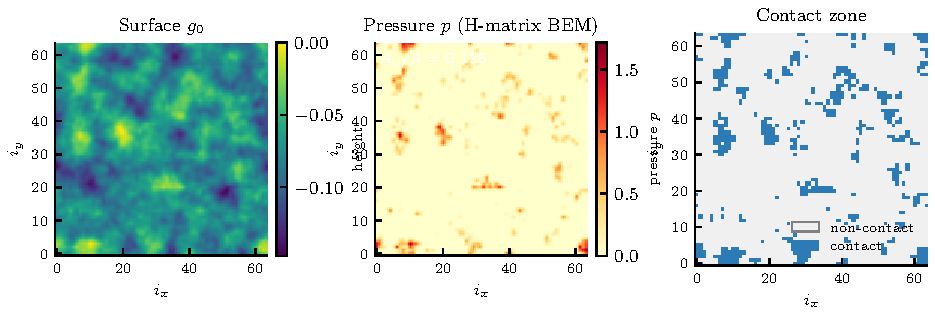
\includegraphics[width=0.96\linewidth]{figures/fig_rough_result.pdf}
  \vspace{0.2em}

  \begin{columns}
  \begin{column}{0.32\textwidth}
    \centering{\small Self-affine surface ($H=0.8$)}
  \end{column}
  \begin{column}{0.32\textwidth}
    \centering{\small $A_c/A = 0.126$,\; mean $p = 0.05\,\Esta$}
  \end{column}
  \begin{column}{0.32\textwidth}
    \centering{\small Contact in 12.6\,\% of elements}
  \end{column}
  \end{columns}
\end{frame}


%% ── Section §4: Performance ─────────────────────────────────────────────────
%% §4 — Performance  (4 slides)
\section{Performance \& Comparison}

%% ── Slide 14: Memory scaling ────────────────────────────────────────────────
\begin{frame}{Memory Scaling: Dense vs.\ H-Matrix}
\begin{columns}[T]
\begin{column}{0.50\textwidth}
  \centering
  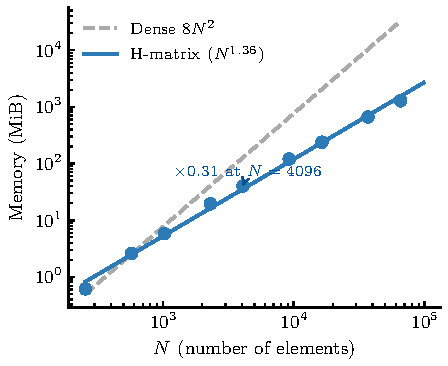
\includegraphics[width=0.96\linewidth]{figures/fig_memory_scaling.pdf}
\end{column}
\begin{column}{0.46\textwidth}
  \begin{block}{Key numbers at $N=4096$ ($N_s=64$)}
    \begin{tabular}{lc}
      \toprule
      Quantity & Value \\
      \midrule
      Dense storage & 128\,MiB \\
      H-matrix storage & 40\,MiB \\
      \textbf{Compression} & \textbf{0.31$\times$} \\
      Dense blocks & 2\,116 \\
      Low-rank blocks & 6\,900 \\
      Avg.\ rank $k$ & 11 \\
      \bottomrule
    \end{tabular}
  \end{block}
  \vspace{0.3em}
  At $N_s=256$ ($N=65\,536$):\\
  H-matrix: 1.3\,GB \quad vs.\quad
  Dense: \alert{34\,GB}
  \vspace{0.2em}

  Fit exponent $\approx N^{1.45}$ in practice
  (target $O(N\log^2 N) \approx N^{1.28}$ at $N\!=\!4096$)
\end{column}
\end{columns}
\end{frame}

%% ── Slide 15: Timing scaling ────────────────────────────────────────────────
\begin{frame}{Timing Scaling: Assembly \& Matvec vs.\ $N$}
\begin{columns}[T]
\begin{column}{0.50\textwidth}
  \centering
  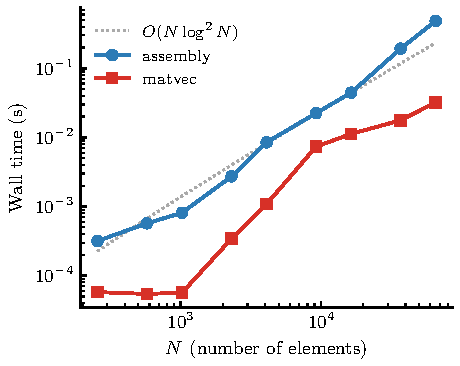
\includegraphics[width=0.96\linewidth]{figures/fig_timing_scaling.pdf}
\end{column}
\begin{column}{0.46\textwidth}
  \begin{block}{Measured wall times (20-core Xeon)}
    \centering
    \begin{tabular}{rrr}
      \toprule
      $N_s$ & Assembly & Matvec \\
      \midrule
       64 &   7\,ms  &  0.6\,ms \\
      128 &  44\,ms  &  11\,ms \\
      256 & 484\,ms  &  32\,ms \\
      \bottomrule
    \end{tabular}
  \end{block}
  \vspace{0.4em}
  \begin{itemize}
    \item Assembly parallelised with OpenMP
    \item Matvec: 9\,016 block GEMVs
      (independent $\to$ OpenMP)
    \item Both roughly $O(N\log^2 N)$
    \item Matvec dominated by low-rank
      blocks ($k\approx11$)
  \end{itemize}
\end{column}
\end{columns}
\end{frame}

%% ── Slide 16: Comparison with Tamaas ────────────────────────────────────────
\begin{frame}{Comparison with Tamaas (Non-Periodic)}
\begin{columns}[T]
\begin{column}{0.52\textwidth}
  \centering
  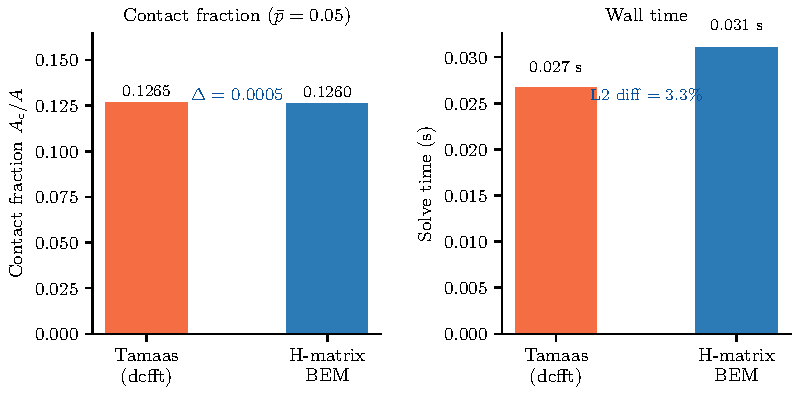
\includegraphics[width=0.96\linewidth]{figures/fig_tamaas_comparison.pdf}
\end{column}
\begin{column}{0.44\textwidth}
  \begin{block}{Summary ($N_s=64$, $\pbar=0.05$)}
    \begin{tabular}{lcc}
      \toprule
      Metric & Tamaas & BEM \\
      \midrule
      $A_c/A$ & 0.1265 & 0.1260 \\
      $|\Delta A_c/A|$ & \multicolumn{2}{c}{0.0005} \\
      $\langle p\rangle / \pbar - 1$ & $<10^{-14}$ & $<10^{-14}$ \\
      Iters & 33 & 26 \\
      $\|p_\mathrm{BEM}-p_\mathrm{T}\|/\|p_\mathrm{T}\|$ &
        \multicolumn{2}{c}{3.3\,\%} \\
      \bottomrule
    \end{tabular}
  \end{block}
  \vspace{0.3em}
  \small
  The 3.3\,\% L2 difference is dominated by\\
  Gibbs-like near-field errors in Tamaas\\
  dcfft operator ($\pm2$--$8$\,\% at $r=1$--$3h$),\\
  \emph{not} by the H-matrix approximation.
\end{column}
\end{columns}
\end{frame}

%% ── Slide 17: Conclusions ───────────────────────────────────────────────────
\begin{frame}{Conclusions}
\begin{columns}[T]
\begin{column}{0.55\textwidth}
  \textbf{Delivered}:
  \begin{itemize}
    \item C++17 H-matrix BEM library
      (\texttt{libhmatrix\_contact + Python module})
    \item Love element kernel (exact, $O(1)$ lookup)
    \item Quad-tree + ACA ($\varepsilon_{\rm aca}=10^{-6}$)
    \item Polonsky--Keer PCG solver
    \item OpenMP-parallel assembly \& matvec
  \end{itemize}

  \vspace{0.5em}
  \textbf{Validated}:
  \begin{itemize}
    \item Hertz: $a_{\rm num}/a = 1.016$,
      $p_{\rm max}/p_0 = 0.998$
    \item H-matvec vs.\ dense: $<10^{-5}$ rel.\ L2
    \item Rough contact vs.\ Tamaas: $|\Delta A_c|=0.0005$
  \end{itemize}
\end{column}
\begin{column}{0.40\textwidth}
  \begin{block}{Outlook}
    \begin{itemize}
      \item Larger grids via MPI\\
        ($N_s \sim 10^3$, $N\sim10^6$)
      \item Plasticity (Mindlin--Deresiewicz)
      \item Adhesion (JKR / DMT)
      \item 3D bodies (volume BIE)
      \item Non-conforming surface meshes
    \end{itemize}
  \end{block}
  \vspace{0.4em}
  \small
  Code: \texttt{Hcontact/} \\
  Build:
  \begin{itemize}
    \item \texttt{cmake -S . -B build}\\
      \texttt{\;\;-DCMAKE\_CXX\_COMPILER=/usr/bin/g++}
    \item \texttt{cmake --build build -j}
    \item \texttt{ctest --test-dir build}
  \end{itemize}
\end{column}
\end{columns}
\end{frame}


\end{document}
